A lake stage is a dependent variable of the simulation, but by default the Lake (LAK) Package does not add its equations to the groundwater flow matrix: the stage is solved in the outer iteration. An adjoint solution built from the flow matrix alone therefore treats the stage as fixed, and reports only the part of a sensitivity that travels through the aquifer. This chapter describes how the lake water balance is brought into the adjoint system.

\section*{The fixed-stage error}

Consider pumping near a lake. The heads beneath the lake fall, which increases the leakage from the lake to the aquifer; the lake stage then falls too, which reduces the leakage that the lower heads would otherwise have drawn. A sensitivity computed with the stage held fixed captures the first effect and not the second, so it does not answer the question a capture analysis asks \citep[for example,][]{leake2010,barlow2012}.

The stage cannot simply be added to the flow matrix, because \mf{} does not put it there. Instead the adjoint system is extended.

\section*{Bordered system}

Let $\mathbf{h}$ be the cell heads and $\mathbf{s}$ the stages of the lakes whose stage is free to move. Write the aquifer residual as $\mathbf{r}$, as in equation~\ref{eqn:residual}, and the lake water balance as $\mathbf{r}_{L}$. The two sets of equations together are

\begin{equation}
	\label{eqn:lak-bordered}
	\begin{bmatrix}
		\dfrac{\partial \mathbf{r}}{\partial \mathbf{h}} &
		\dfrac{\partial \mathbf{r}}{\partial \mathbf{s}} \\[2ex]
		\dfrac{\partial \mathbf{r}_{L}}{\partial \mathbf{h}} &
		\dfrac{\partial \mathbf{r}_{L}}{\partial \mathbf{s}}
	\end{bmatrix}
	\begin{bmatrix} \mathbf{h} \\ \mathbf{s} \end{bmatrix}
	=
	\begin{bmatrix} \mathbf{b} \\ \mathbf{b}_{L} \end{bmatrix}.
\end{equation}

The leading block is the matrix $\left[ \mathbf{A} \right]^{k}$ of equation~\ref{eqn:forward}. The other three blocks add one row and one column per free lake, which is why this is called a bordered matrix: the original system sits inside a border one equation deep. The adjoint problem is the transpose of equation~\ref{eqn:lak-bordered}, and its solution has one extra entry per lake alongside the usual one per cell.

A lake with a specified stage contributes no unknown and is left out of the border, as is an inactive lake.

\subsection*{Connection terms}

Each lake-aquifer connection carries a conductance $C_{n,\ell}$ (L$^{2}$T$^{-1}$) between cell $n$ and lake $\ell$. The exchange depends on both the head in the cell and the stage of the lake, giving the off-diagonal blocks

\begin{equation}
	\label{eqn:lak-offdiag}
	\frac{\partial r_{n}}{\partial s_{\ell}} = C_{n,\ell}, \qquad
	\frac{\partial r_{L,\ell}}{\partial h_{n}} = \mathrm{HCOF}_{n},
\end{equation}

\noindent summed over the connections between cell $n$ and lake $\ell$, and the conductance also accumulates on the lake's own diagonal.

The two halves of equation~\ref{eqn:lak-offdiag} are not written the same way, and the difference matters. A lake perched above the water table leaks at a rate set by its bed rather than by the head beneath it. \mf{} marks that state by leaving \texttt{HCOF} at zero for the connection while the exchange still follows the stage. Using the conductance on both sides gives a lake perched above a falling water table a head sensitivity it does not have; using \texttt{HCOF} on the head side and the conductance on the stage side reproduces the two cases with one expression.

\subsection*{Storage and surface area}

A transient step adds the change in lake storage to the diagonal, $\partial V / \partial s$ divided by the time step length, where $V$ is the lake volume (L$^{3}$) and $s$ is the lake stage (L). A steady-state step adds nothing.

A lake whose surface area grows with stage evaporates more as it rises and catches more rain, and those act in opposite senses, so the diagonal also carries

\begin{equation}
	\label{eqn:lak-surface}
	\left( E - P \right) \frac{\partial S_{A}}{\partial s},
\end{equation}

\noindent where $E$ is the evaporation rate (LT$^{-1}$), $P$ the rainfall rate (LT$^{-1}$), and $S_{A}$ the lake surface area (L$^{2}$). Where the lake geometry is given as a table of stage against volume and area, the derivatives $\partial V / \partial s$ and $\partial S_A / \partial s$ are the slopes of the interval of the table holding the current stage, matching the interpolation \mf{} performs.

As with the aquifer, the lake storage term also couples one time step to the next, and the stage part of the adjoint solution is carried backward in the same way. An instantaneous measure, for which the time steps are independent, does not carry it (Chapter~\ref{ch:instantaneous}).

\subsection*{Outlets}

An outlet discharges over an invert according to its type: a specified rate, a Manning rating, or a weir. Each is a power of the depth $d$ over the invert, so the derivative follows from the discharge itself,

\begin{equation}
	\label{eqn:lak-outlet}
	\frac{\partial Q_{\mathrm{out}}}{\partial s} = \gamma
	\frac{Q_{\mathrm{out}}}{d}, \qquad
	\gamma = \begin{cases}
		0, & \text{specified rate}, \\
		5/3, & \text{Manning}, \\
		3/2, & \text{weir}.
	\end{cases}
\end{equation}

Writing the derivative in terms of the reported discharge rather than recomputing the rating avoids reproducing the roughness, width, and slope of the outlet. Where an outlet discharges from one lake into another, the derivative also appears off the diagonal, coupling the two lake rows.

Very close to the invert \mf{} smooths the rating to zero. That smoothing is not reproduced here, so an outlet with a depth below $10^{-6}$ in model length units is treated as carrying no flow.

\section*{Verification}

\begin{figure}[htb]
	\centering
	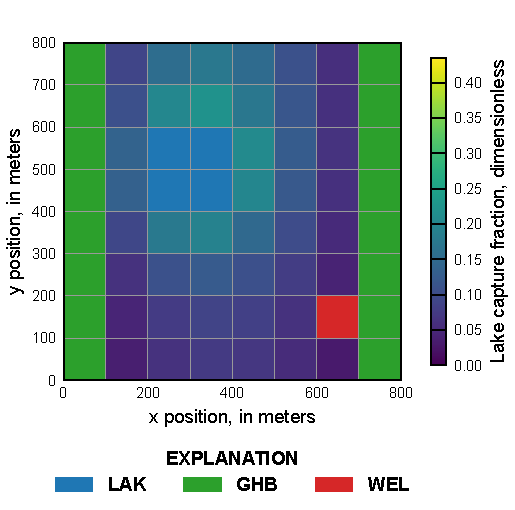
\includegraphics{Figures/lake-capture.pdf}
	\caption{Lake capture fraction for the model the lake tests use, the
	fraction of a withdrawal at a cell that is drawn from the lake rather than
	from storage or from another boundary, for the second model layer, in which
	it is largest. LAK marks the cells the lake connects to, GHB the
	general-head boundaries that hold the heads at the left and right edges of
	the model, and WEL the pumped cell. The lake is incised into the top layer,
	which is inactive beneath it, and reaches the aquifer through one vertical
	connection per cell into the layer shown, so the capture is the response the
	water balance of this chapter describes, without the approximations noted at
	the end.}
	\label{fig:lake-capture}
\end{figure}

A lake sitting in a two layer model was pumped from a cell away from it, and the resulting change in lake exchange compared with the difference between two forward runs. The adjoint reports a capture of $-3.4232 \times 10^{-2}$ against a two-run difference of $-3.4258 \times 10^{-2}$, a difference of 0.08 percent. The model is the one the lake tests use, so the figure shows the lake whose behavior those tests check. Capture fractions across that model are shown in figure~\ref{fig:lake-capture}. With the stage held fixed the adjoint reported a lake capture of $-4.1 \times 10^{-3}$ against a two-run difference of $-4.6 \times 10^{-3}$, an error of about a factor of two in the part of the response the stage carries. Solving the water balance with the flow equations reduced the discrepancy to $-5 \times 10^{-4}$.

The residual discrepancy is not numerical. It is accounted for by two couplings that remain outside the border: inflow routed to the lake by the Water Mover (MVR) Package, which follows the state of the package supplying it, and the dependence of a horizontal connection's conductance on the saturated fraction of the cell it connects to.
